\documentclass{article}
\usepackage{graphicx} % Required for inserting images
\usepackage{subcaption}
\usepackage{amsmath, amssymb, booktabs}
\usepackage{hyperref}
\usepackage{comment}
\graphicspath{ {../imgs/} }

\title{Three for Two}
\author{Johnathan Ferdinand, Devina Gera, Archimedes Li, Henry Liu, \\Katherine Shi, Sam Stevens}
\date{\today}
\begin{document}
\maketitle

\section{Introduction}

\[
\text{Returns}_t = \beta_0 + \beta_1,\text{Returns}_{t-1}.
\]

\[
r_t = \beta_0 + \beta_1r_{t-1}.
\]

Our model is a generalized linear regression model that uses the logit link function to perform a binary classification of raisins to either the Kecimen or Besni class. Our model uses seven independent variables, further detailed in the data description, to predict a probability as following:

$$\ln \left( \frac{p}{1-p}\right) = \beta_0 + \sum_{i=1}^{7} \beta_i X_i$$

where we solve for $p$, the probability that a raisin belongs to the Besni class. Our model then compares the probabilities $p$ and $1-p$, classifying the instance as Kecimen if $1-p > p$ and Besni otherwise.

We choose the logit function as our link function due to its conversion of a problem involving linear parameters to a binary classification output by modeling probabilities for two classes. Our model, as with most linear models, lacks complexity as opposed to an alternative solution, such as one using neural networks. As such, we chose a dataset with simple parameters that have a linear relation to the output to amend for this fact.

The R packages that we used were \texttt{caTools, tidyverse, caret, ggplot2, dplyr, pROC, ggfortify}

Our model was trained on 720 instances and performed with $87.2\%$ accuracy on the testing set of 180 instances.

\section{Data Description}
Our dataset is for raisin classification between Kecimen and Besni raisin types.  The dataset extracts 7 different features from 900 images of raisins, with 450 of each type of raisin.
Area - Gives the number of pixels within the boundaries of the raisin.
Major axis length - Gives the pixel length of the main axis, which is the longest line that can be drawn on the raisin.
Minor axis length - Gives the pixel length of the small axis, which is the shortest line that can be drawn on the raisin.
Eccentricity - It gives a measure of the eccentricity of the ellipse, which has the same moments as raisins.  Values closer to 0 indicate the raisin is more circular, and values closer to 1 indicate that the raisin is more elongated.
Convex area - Gives the number of pixels of the smallest convex shell of the region formed by the raisin.
Extent - Gives the ratio of the region formed by the raisin to the total pixels in the bounding box.  Ranges from 0 to 1.
Perimeter - It measures the environment by calculating the distance between the boundaries of the raisin and the pixels around it.

\section{Analysis}
We first scrambled the data, because the raisin data was sorted by raisin type. We then used 80\% of the data to train our model and the remaining 20\% for testing. \\
These are the coefficients for our model:
\begin{verbatim}
Coefficients:
                  Estimate Std. Error z value Pr(>|z|)   
(Intercept)     -3.164e+00  7.495e+00  -0.422  0.67296   
Area             5.295e-04  1.065e-04   4.970 6.70e-07 **
MajorAxisLength -4.471e-02  1.735e-02  -2.577  0.00997 **
MinorAxisLength -8.355e-02  2.923e-02  -2.858  0.00426 **
Eccentricity    -2.472e+00  5.232e+00  -0.473  0.63654   
ConvexArea      -4.389e-04  9.095e-05  -4.826 1.39e-06 **
ConvexArea      -4.389e-04  9.095e-05  -4.826 1.39e-06 **
Extent          -1.127e+00  3.015e+00  -0.374  0.70857   
Perimeter        3.480e-02  6.876e-03   5.060 4.19e-07 **
\end{verbatim}
The eccentricity, Extent, and Intercept are not strong predictors, as made apparent by their large $P$ values, and by their logistic regression plots (Figure \ref{fig:lr})
\clearpage
\begin{figure}[ht]
	\centering
	\begin{subfigure}{0.4\textwidth}
		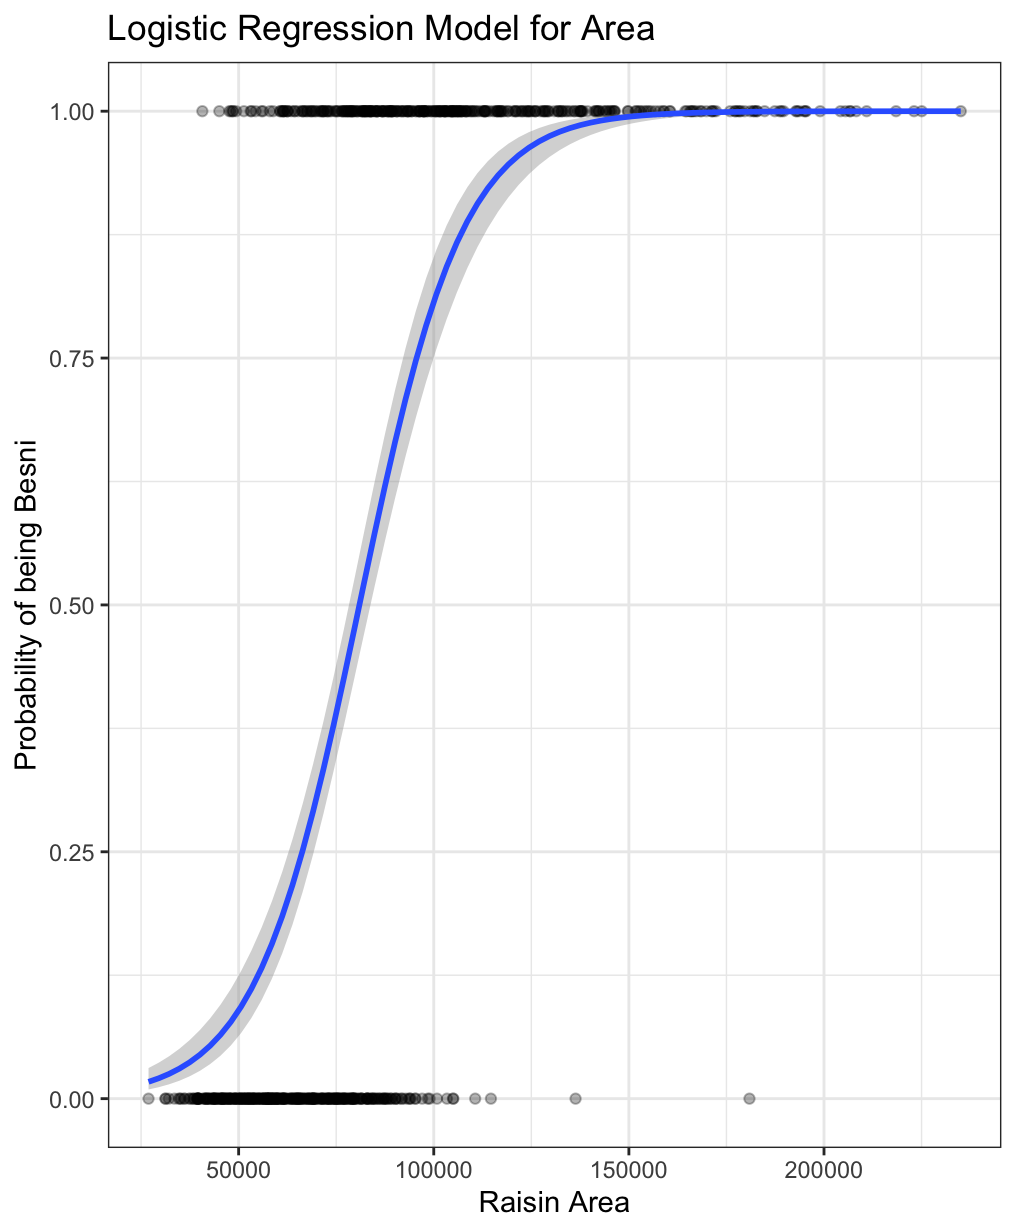
\includegraphics[width=\textwidth]{area_plot}
		\caption{Logistic regression model of the probability of being Besni as a function of raisin area.}
		\label{fig:area}
	\end{subfigure}
	\hfill
	\begin{subfigure}{0.4\textwidth}
		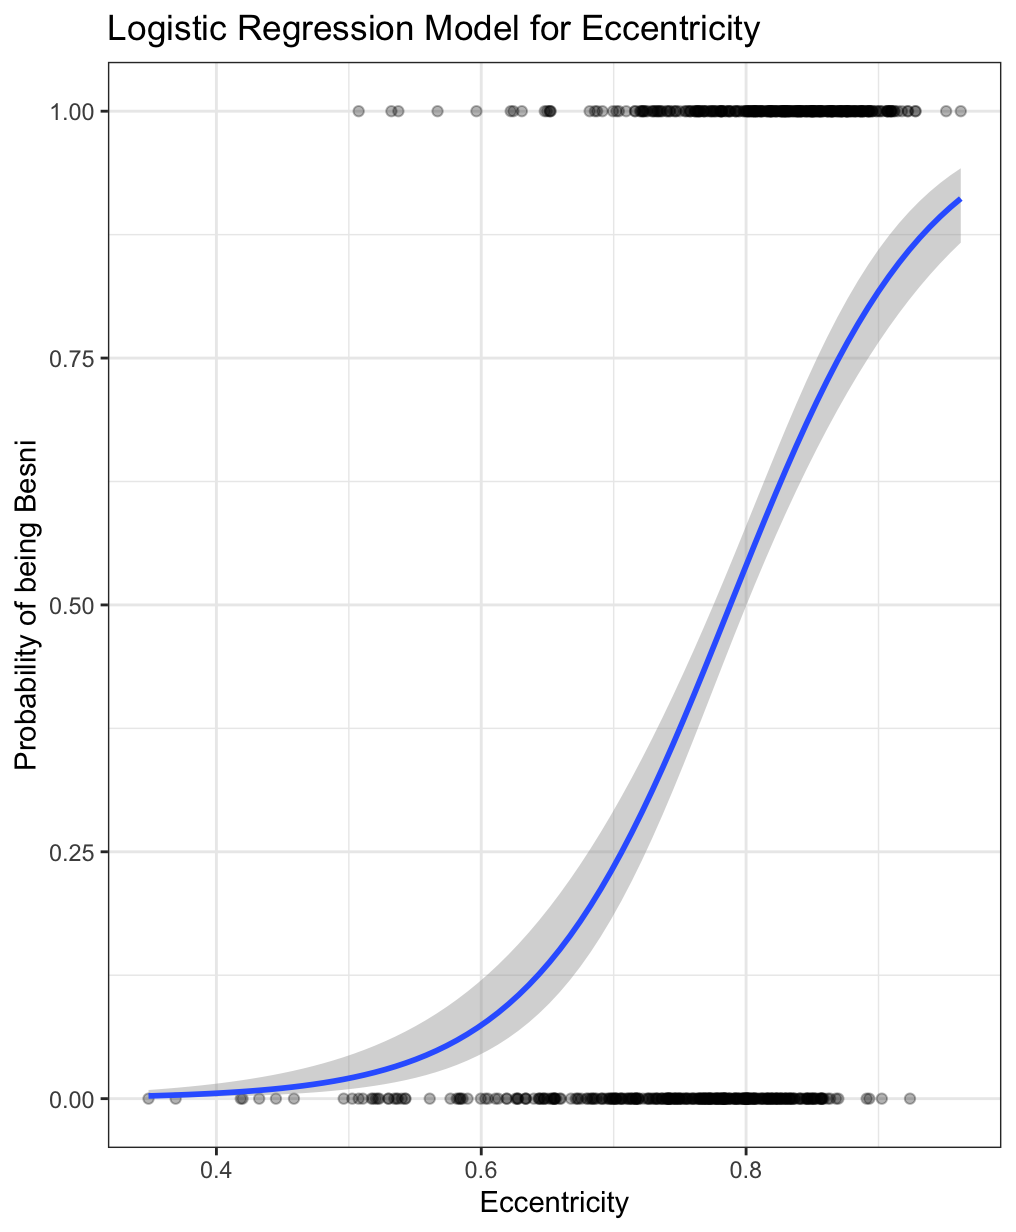
\includegraphics[width=\textwidth]{ecc_plot}
		\caption{Logistic regression model of probability of being Besni as function of eccentricity.}
		\label{fig:ecc}
	\end{subfigure}
	\caption{The slope of the area plot (figure \subref{fig:area}) being steeper than that of the eccentricity plot (figure \subref{fig:ecc}) indicates that area has a larger impact on the probability of the raisin being Besni, which is consistant with the coefficient table.}
	\label{fig:lr}
\end{figure}
Our diagonal plot for our model is shown in (Figure \ref{fig:diag})
\begin{figure}[!ht]
	\centering
	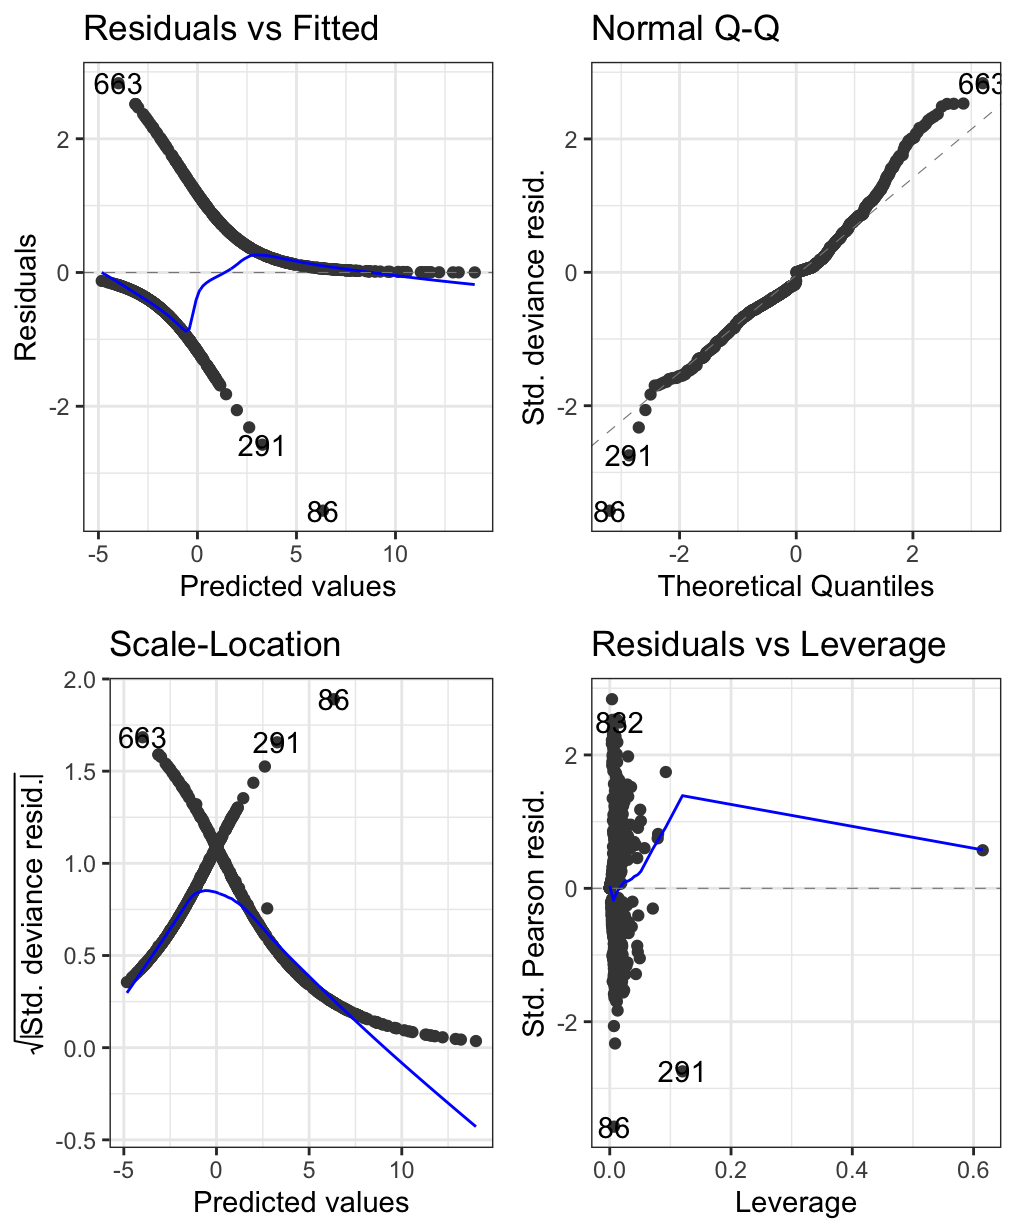
\includegraphics[width=0.5\textwidth]{diagonal_plots}
\caption{Diagonal plot for our model.}
\label{fig:diag}
\end{figure}

\clearpage
Clockwise from the top left(Figure \ref{fig:diag}):The Residual vs Fitted plot shows a clear pattern to the residuals and fitted points with an asymptote, so the model does not fit the data well.\\
The Normal Q-Q plot tells us that the data is normally distributed because the data mostly follows the $y=x$ line.\\
In the Scale-Location plot, the blue line is not horizontal and has a spike near 0 so the equal variance assumption is violated.\\
The Residual vs Leverage plot shows no high leverage points with large residuals. \\
The ROC curve is shown in Figure \ref{fig:roc}. With an AUC of 0.9434, the model does well at classifying observations as being more like Kecimen or Besni.
\begin{figure}[ht]
	\centering
	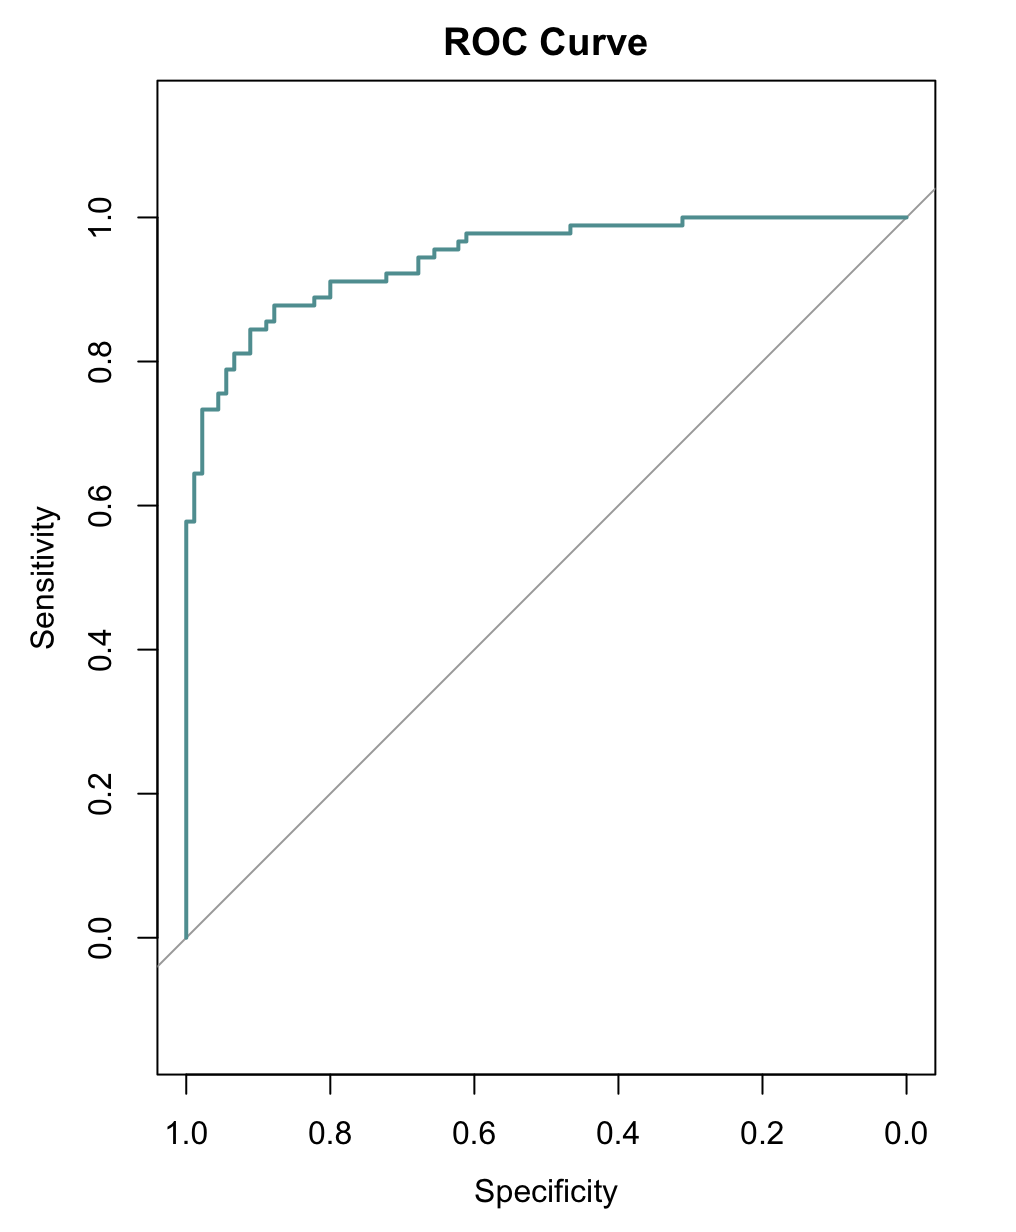
\includegraphics[width=0.75\textwidth]{roc_curve}
\caption{ROC curve for our model}
\label{fig:roc}
\end{figure} \\
Our code can be found in Appendix A.
\clearpage



\section{Model Evaluation}

To ensure our model is optimal for classifying raisins into the Besni and Kecimen classes, we performed subset selection, assessed the model using various statistical tests, and evaluated prediction accuracy using multiple performance metrics.

\hfill\break

Initially, our model included all seven independent variables: \textit{Area}, \textit{MajorAxisLength}, \textit{MinorAxisLength}, \textit{Eccentricity}, \textit{ConvexArea}, \textit{Extent}, and \textit{Perimeter}. However, not all predictors significantly contributed to the model, as indicated by their p-values in the coefficient summary. Specifically, \textit{Eccentricity}, \textit{Extent}, and the intercept had large p-values, implying weak predictive power. We performed backward elimination, iteratively removing these non-significant predictors to improve model performance. The final model included the following predictors:

\begin{itemize}
\item \textbf{Area} ($p = 6.70 \times 10^{-7}$)
\item \textbf{MajorAxisLength} ($p = 0.00997$)
\item \textbf{MinorAxisLength} ($p = 0.00426$)
\item \textbf{ConvexArea} ($p = 1.39 \times 10^{-6}$)
\item \textbf{Perimeter} ($p = 4.19 \times 10^{-7}$)
\end{itemize}

This refined model was used for further evaluation and prediction.
\hfill\break

To validate the model's fit, we analyzed the following diagnostic plots:

\begin{itemize}
\item \textbf{Residuals vs. Fitted:} A pattern in residuals indicated some level of model misfit, but no severe violations of assumptions were observed.
\item \textbf{Normal Q-Q Plot:} The residuals were approximately normally distributed, confirming the model's appropriateness.
\item \textbf{Scale-Location Plot:} A non-horizontal trend suggested a mild violation of homoscedasticity.
\item \textbf{Residuals vs. Leverage:} No significant high-leverage points with large residuals were detected, suggesting no influential outliers affected the model.
\end{itemize}

\hfill\break

Additionally, we computed the Receiver Operating Characteristic (ROC) curve to evaluate classification performance. The model achieved an Area Under the Curve (AUC) of 0.9434, indicating strong discriminatory power between the two raisin types.


We assessed the predictive accuracy of the final model using the test dataset. The confusion matrix results were:

\newpage

\begin{table}[h]
\centering
\begin{tabular}{c|c c}
\toprule
\textbf{Predicted} & \textbf{Actual Kecimen} & \textbf{Actual Besni} \\
\midrule
Kecimen & $TP = 82$ & $FN = 15$ \\
Besni & $FP = 8$ & $TN = 75$ \\
\bottomrule
\end{tabular}
\caption{Confusion Matrix of Model Predictions}
\label{tab:conf_matrix}
\end{table}

Using this, we computed:
\begin{itemize}
\item \textbf{Accuracy:} $\frac{TP + TN}{TP + TN + FP + FN} = 87.22\%$
\item \textbf{Precision (for Kecimen class):} $\frac{TP}{TP + FP} = 91.11\%$
\item \textbf{Recall (for Kecimen class):} $\frac{TP}{TP + FN} = 84.53\%$
\item \textbf{Precision (for Besni class):} $\frac{TN}{TN + FN} = 83.33\%$
\item \textbf{Recall (for Besni class):} $\frac{TN}{TN + FP} = 90.36\%$
\end{itemize}

With an accuracy of 87.22\%, the model effectively differentiates between the two raisin types. The high precision and recall values suggest that false positives and false negatives are minimal, reinforcing the robustness of our logistic regression model.

Finally, we used the trained model to predict new instances. Given an input raisin image with extracted features, the model calculates the probability $p$ of being Besni and classifies it accordingly. The decision rule is:
\begin{equation}
\text{Class} = \begin{cases}
\text{Besni}, & \text{if } p > 0.5 \\
\text{Kecimen}, & \text{otherwise.}
\end{cases}
\end{equation}

These results confirm that our logistic regression model, refined through subset selection and validated with statistical tests, performs well in classifying raisin types with high accuracy.


\section{Conclusion}

In summary, our generalized linear regression model using the logit link function effectively classifies raisins into Kecimen or Besni classes based on seven distinct features extracted from images. The model leverages simple, linear relationships between these features and the classification outcome, making it suitable for this specific dataset.

One of the positive aspects of our model is its simplicity and interpretability. The straightforward nature of the model makes it accessible for users who may not be familiar with more complex machine learning techniques. Additionally, the model is computationally efficient, allowing for quick training on the dataset. The accuracy of $87.22\%$ achieved on the testing set of 180 instances demonstrates the model's effectiveness in distinguishing between the two raisin types.

However, the model does have some limitations. Its limited complexity means it may not capture more intricate, non-linear relationships within the data, potentially limiting its performance compared to more advanced models like neural networks. Furthermore, the accuracy of the model is highly dependent on the quality and relevance of the selected features. Any noise or irrelevant features can adversely affect the model's performance.

Looking ahead, there are several avenues for future work. Refining the features or including additional relevant features could enhance the model's accuracy. Exploring more complex models, such as neural networks or ensemble methods, could potentially improve classification performance. Implementing cross-validation techniques would also ensure the model's robustness and generalizability across different subsets of the data.

Several factors affect the model's accuracy, including the quality of the images and the precision in feature extraction. The number of instances used for training and testing can impact the model's ability to generalize. Lastly, the choice of features plays a crucial role in determining the model's performance.

Overall, while our model provides a solid foundation for raisin classification, there is room for improvement through more sophisticated techniques and further data analysis.


\begin{thebibliography}{9}

\bibitem{STHDA}
\emph{Logistic regression essentials in R - articles - STHDA}. (2018, November 3). http://www.sthda.com/english/articles/36-classification-methods-essentials/151-logistic-regression-essentials-in-r

\bibitem{Raisin}
\emph{Raisin binary classification}. (2024, February 11). Kaggle. https://www.kaggle.com/datasets/nimapourmoradi/raisin-binary-classification/data


\bibitem{advert}
\emph{SOGA}. (n.d.). https://www.geo.fu-berlin.de/en/v/soga/Basics-of-statistics/Logistic-Regression/Logistic-Regression-in-R---An-Example/index.html


\end{thebibliography}

\section{Appendix A}
\begin{verbatim}
# Load required libraries
library(caTools)
library(tidyverse)
library(caret)
library(ggplot2)
library(dplyr)
library(pROC)
library(ggfortify)

# Load data set
raisins <- read.csv("Raisin_Dataset.csv")
raisins <- na.omit(raisins) # Remove missing values

# Convert Class to binary (Besni = 1, Kecimen = 0)
raisins$Class <- ifelse(raisins$Class == "Besni", 1, 0)

# Shuffle data
set.seed(37)
raisins <- raisins[sample(nrow(raisins)), ]

# Split into training and test set
split <- sample.split(raisins$Class, SplitRatio = 0.8)

train <- subset(raisins, split == TRUE)
test <- subset(raisins, split == FALSE)

# Model
model <- glm(Class ~ Area + MajorAxisLength + MinorAxisLength + 
                 Eccentricity + ConvexArea + Extent + Perimeter, 
               data = train, 
               family = "binomial")

summary(model)

dev.new()
autoplot(model)

# Predictions
pred <- predict(model, test, type = "response")
pred_class <- ifelse(pred > 0.5, "Besni", "Kecimen")

# Confusion Matrix
conf_matrix <- table(Predicted = pred_class, Actual = test$Class)
print(conf_matrix)

train.data <- train %>%
  mutate(prob = predict(model, type = "response"))

dev.new()
area_plot <- ggplot(train.data, aes(x = Area, y = Class)) +
  geom_point(alpha = 0.3) +  
  geom_smooth(method = "glm", method.args = list(family = "binomial")) +
  labs(
    title = "Logistic Regression Model for Area",
    x = "Raisin Area",
    y = "Probability of being Besni"
  )

print(area_plot)

dev.new()
ecc_plot <- ggplot(train.data, aes(x = Eccentricity, y = Class)) +
  geom_point(alpha = 0.3) +  
  geom_smooth(method = "glm", method.args = list(family = "binomial")) +
  labs(
    title = "Logistic Regression Model for Eccentricity",
    x = "Eccentricity",
    y = "Probability of being Besni"
  )

print(ecc_plot)

# ROC curve
roc_curve <- roc(test$Class, pred)
dev.new()
plot(roc_curve, col = "cadetblue", main = "ROC Curve")
auc_value <- auc(roc_curve)
cat("AUC:", auc_value, "\n")

# Feature Importance
importance <- summary(model)$coefficients[, "Estimate"]
importance_df <- data.frame(Feature = names(importance), Estimate = importance)
dev.new()
ggplot(importance_df, aes(x = reorder(Feature, Estimate), y = Estimate)) +
  geom_bar(stat = "identity", fill = "pink") +
  coord_flip() +
  labs(title = "Feature Importance",
       x = "Feature",
       y = "Coefficient Estimate")
\end{verbatim}
\end{document}

